% Koko
\documentclass[blue,normal,cn]{elegantnote}
\usepackage{array}
\usepackage{courier}
\usepackage{xcolor}
\usepackage{zhnumber}
\usepackage{ulem}
\usepackage{float}

\definecolor{light-gray}{gray}{0.95}
\newcommand{\code}[1]{\colorbox{light-gray}{\texttt{#1}}}
\newfontfamily\courier{Courier New}
\lstset{linewidth=1.1\textwidth,
	numbers=left,
	basicstyle=\small\courier,
	numberstyle=\tiny\courier,
	keywordstyle=\color{blue}\courier,
	commentstyle=\it\color[cmyk]{1,0,1,0}\courier, 
	stringstyle=\it\color[RGB]{128,0,0}\courier,
	frame=single,
	backgroundcolor=\color[RGB]{245,245,244},
	breaklines,
	extendedchars=false, 
	xleftmargin=2em,xrightmargin=2em, aboveskip=1em,
	tabsize=4, 
	showspaces=false
	basicstyle=\small\courier
}
\title{实验 4: 使用 MIPS 指令实现冒泡排序法}
\version{$\aleph$}
\date{\zhtoday}

\begin{document}
\author{
    \begin{tabular}[t]{c}
        于海鑫 \\
        2017211240
    \end{tabular}
}
\maketitle

\section{实验目的}
\begin{enumerate}
    \item 掌握静态调度方法
    \item 增强汇编语言编程能力
    \item 学会使用模拟器中的定向功能进行优化
\end{enumerate}

\section{实验平台}

实验平台采用指令级和流水线操作级模拟器 \code{MIPSsim}。

\section{实验内容和步骤}

\begin{enumerate}[wide=0pt, listparindent=2em, parsep=0pt]
    \item 自行编写一个实现冒泡排序的汇编程序,该程序要求可以实现对一维整数数组进行冒泡排序。
    \item 启动 MIPSsim。
    \item 载入自己编写的程序,观察流水线输出结果。
    \item 使用定向功能再次执行代码,与刚才执行结果进行比较,观察执行效率的不同。
    \item 采用静态调度方法重排指令序列,减少相关,优化程序。
    \item 对优化后的程序使用定向功能执行,与刚才执行结果进行比较,观察执行效率的不同。
\end{enumerate}

\section{冒泡排序}

\subsection{代码}
冒泡排序几乎是刻在大家 DNA 里面的程序了吧,在此就不再展示其 C 代码了,我们的程序的签名如下:

\begin{lstlisting}[language=C]
void bubble(int *arr, int n);
\end{lstlisting}

我们要做的就是把 DNA 里面的冒泡排序代码转换成汇编的,结果如下(需要注意 MIPS 的\href{https://courses.cs.washington.edu/courses/cse410/09sp/examples/MIPSCallingConventionsSummary.pdf}{\textbf{调用约定}})

\lstinputlisting{naive_bubble.s}

\subsection{运行结果}

\subsubsection{未开启定向功能时}

\begin{lstlisting}
  汇总:
    执行周期总数:981
    ID段执行了492条指令

  硬件配置:
    内存容量:4096 B
    加法器个数:1		执行时间(周期数):6
    乘法器个数:1		执行时间(周期数)7		
    除法器个数:1		执行时间(周期数)10		
    定向机制:不采用

  停顿(周期数):
    RAW停顿:365		占周期总数的百分比:37.20693%
    其中:
      load停顿:110		占所有RAW停顿的百分比:30.13699%
      浮点停顿:0		占所有RAW停顿的百分比:0%
    WAW停顿:0		占周期总数的百分比:0%
    结构停顿:0		占周期总数的百分比:0%
    控制停顿:123		占周期总数的百分比:12.53823%
    自陷停顿:0		占周期总数的百分比:0%
    停顿周期总数:488	占周期总数的百分比:49.74516%

  分支指令:
    指令条数:122		占指令总数的百分比:24.79675%
    其中:
      分支成功:56		占分支指令数的百分比:45.90164%
      分支失败:67		占分支指令数的百分比:54.91803%

  load/store指令:
    指令条数:221		占指令总数的百分比:44.9187%
    其中:
      load:111		占load/store指令数的百分比:50.22625%
      store:110		占load/store指令数的百分比:49.77375%

  浮点指令:
    指令条数:0		占指令总数的百分比:0%
    其中:
      加法:0		占浮点指令数的百分比:0%
      乘法:0		占浮点指令数的百分比:0%
      除法:0		占浮点指令数的百分比:0%

  自陷指令:
    指令条数:1		占指令总数的百分比:0.203252%
\end{lstlisting}

时钟周期图如下:

\begin{figure}[H]
    \centering
    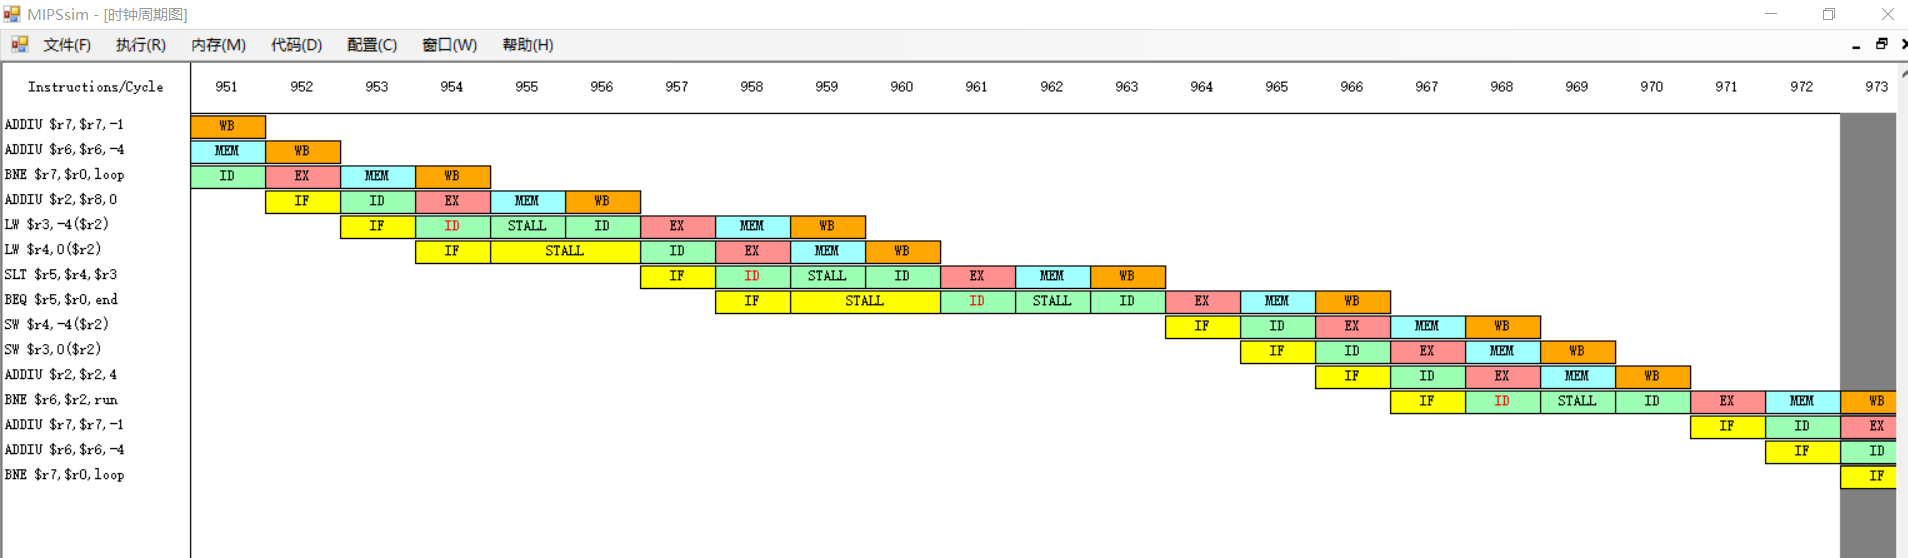
\includegraphics[width=.8\textwidth]{fig/naive_bubble.png}
    \caption{时钟周期图}
    \label{fig:naive_prod}
\end{figure}

\subsubsection{开启定向功能后}

\begin{lstlisting}
    汇总:
    执行周期总数:782
    ID段执行了492条指令

  硬件配置:
    内存容量:4096 B
    加法器个数:1		执行时间(周期数):6
    乘法器个数:1		执行时间(周期数)7		
    除法器个数:1		执行时间(周期数)10		
    定向机制:采用

  停顿(周期数):
    RAW停顿:166		占周期总数的百分比:21.22762%
    其中:
      load停顿:55		占所有RAW停顿的百分比:33.13253%
      浮点停顿:0		占所有RAW停顿的百分比:0%
    WAW停顿:0		占周期总数的百分比:0%
    结构停顿:0		占周期总数的百分比:0%
    控制停顿:123		占周期总数的百分比:15.7289%
    自陷停顿:0		占周期总数的百分比:0%
    停顿周期总数:289	占周期总数的百分比:36.95652%

  分支指令:
    指令条数:122		占指令总数的百分比:24.79675%
    其中:
      分支成功:56		占分支指令数的百分比:45.90164%
      分支失败:67		占分支指令数的百分比:54.91803%

  load/store指令:
    指令条数:221		占指令总数的百分比:44.9187%
    其中:
      load:111		占load/store指令数的百分比:50.22625%
      store:110		占load/store指令数的百分比:49.77375%

  浮点指令:
    指令条数:0		占指令总数的百分比:0%
    其中:
      加法:0		占浮点指令数的百分比:0%
      乘法:0		占浮点指令数的百分比:0%
      除法:0		占浮点指令数的百分比:0%

  自陷指令:
    指令条数:1		占指令总数的百分比:0.203252%
\end{lstlisting}

时钟周期图如下:

\begin{figure}[H]
    \centering
    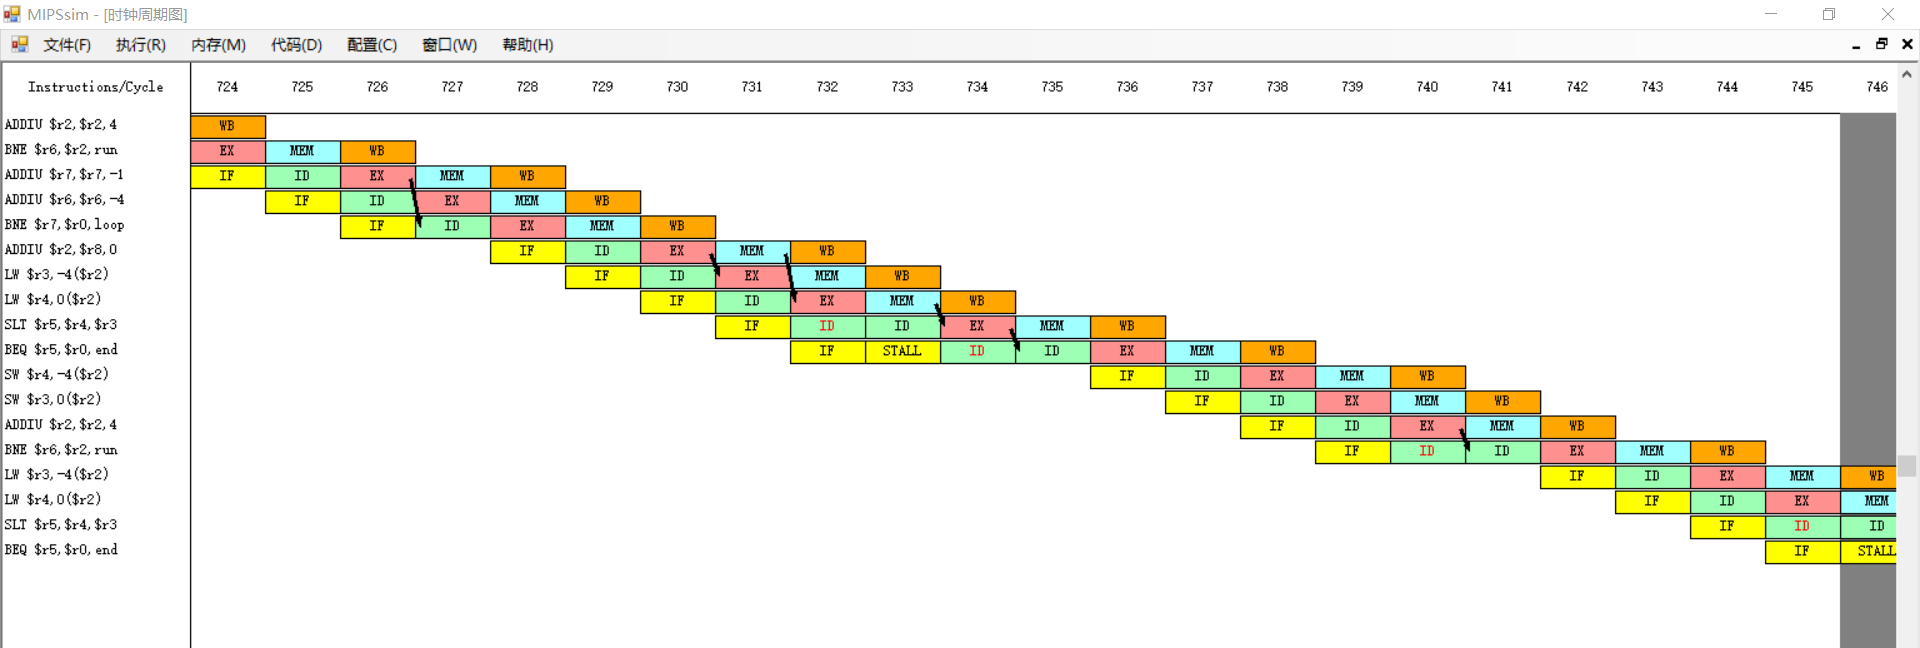
\includegraphics[width=.8\textwidth]{fig/naive_bubble_bypass.png}
    \caption{时钟周期图}
    \label{fig:naive_prod_bypass}
\end{figure}

\section{优化后的冒泡排序}

\subsection{代码}

很遗憾的是,在这里我们的代码可以优化的地方寥寥无几,能修改的只有删掉之前符合语义的 \code{SLT} 指令。修改后的代码如下:

\lstinputlisting{bubble.s}

\subsection{运行结果}

\begin{lstlisting}
  汇总:
    执行周期总数:507
    ID段执行了382条指令

  硬件配置:
    内存容量:4096 B
    加法器个数:1		执行时间(周期数):6
    乘法器个数:1		执行时间(周期数)7		
    除法器个数:1		执行时间(周期数)10		
    定向机制:采用

  停顿(周期数):
    RAW停顿:56		占周期总数的百分比:11.04537%
    其中:
      load停顿:0		占所有RAW停顿的百分比:0%
      浮点停顿:0		占所有RAW停顿的百分比:0%
    WAW停顿:0		占周期总数的百分比:0%
    结构停顿:0		占周期总数的百分比:0%
    控制停顿:68		占周期总数的百分比:13.41223%
    自陷停顿:0		占周期总数的百分比:0%
    停顿周期总数:124	占周期总数的百分比:24.45759%

  分支指令:
    指令条数:67		占指令总数的百分比:17.53927%
    其中:
      分支成功:56		占分支指令数的百分比:83.58209%
      分支失败:12		占分支指令数的百分比:17.91045%

  load/store指令:
    指令条数:221		占指令总数的百分比:57.8534%
    其中:
      load:111		占load/store指令数的百分比:50.22625%
      store:110		占load/store指令数的百分比:49.77375%

  浮点指令:
    指令条数:0		占指令总数的百分比:0%
    其中:
      加法:0		占浮点指令数的百分比:0%
      乘法:0		占浮点指令数的百分比:0%
      除法:0		占浮点指令数的百分比:0%

  自陷指令:
    指令条数:1		占指令总数的百分比:0.2617801%
\end{lstlisting}

时钟周期图如下:

\begin{figure}[H]
    \centering
    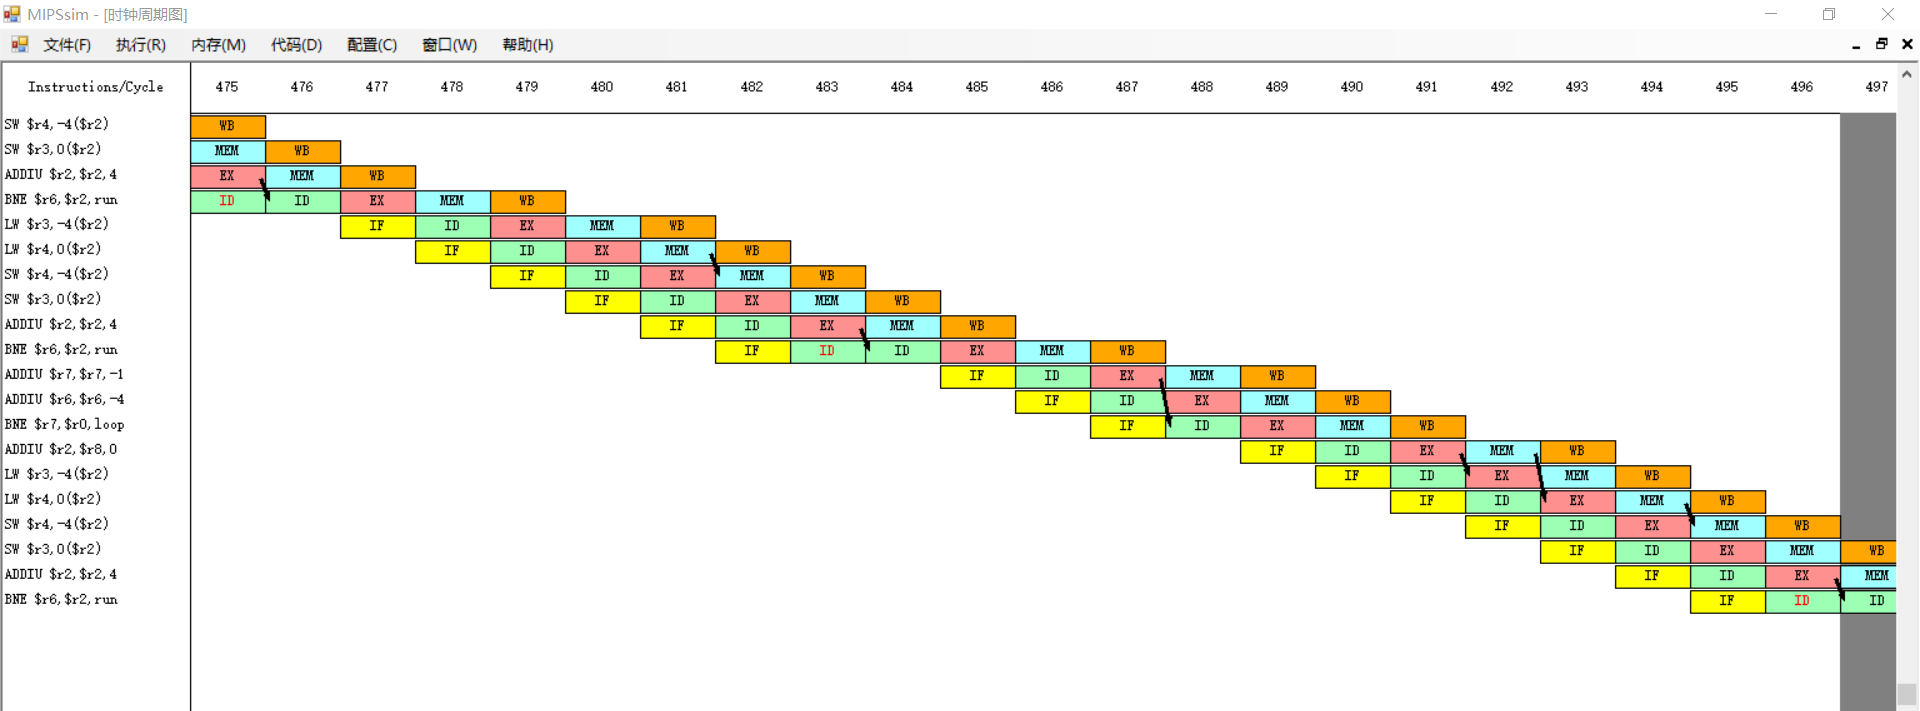
\includegraphics[width=.8\textwidth]{fig/bubble_bypass.png}
    \caption{时钟周期图}
    \label{fig:prod_bypass}
\end{figure}

与之前的代码相比,效率大约是之前的 $782 / 507 = 1.54$ 倍。

\section{实验中的问题与心得}

本次实验主要是人肉模拟编译器做一些简单的优化,本次实验中没有遇到新的问题。

本次的心得大约是通过丧失语义来进行一些更为激烈的优化,我们依然可以很好的进一步榨取 CPU 的性能。

\end{document}